%!TEX root=../paper/paper.tex
\section{Method}\label{sec:ccnn_method}

\PM{R-CNN}
We take the R-CNN \cite{Girshick-CVPR-2014} method as our point of departure.
As summarized in \autoref{fig:rcnn}, R-CNN starts with external region-of-interest proposals (ROIs), which are transformed to canonical size, and classified with a CNN, obtaining multi-class scores for each region.
After all batches of ROIs have been scored, they are post-processed with non-maximal suppression and other bounding box refinement to obtain the final detections.

\PM{Our method}
As summarized in \autoref{fig:combined}, we begin with the same ROI proposals, but first score all proposals with a quick-to-compute feature.
We then select a batch of highly-scoring ROIs and classify them with the CNN -- which is additionally sped up with cascaded structure.
After the batch is scored, we optionally re-score the remaining ROIs, and repeat the process until either time or regions are depleted.
The quick-to-compute feature is used to select batches of regions in a way that orders the regions most likely to contain ground truth objects earlier than other regions.
This process of region selection does not reject regions flat out, but reorders them to be processed later.

\PM{Region order}
We found that simply sorting the regions by score and taking batches in that sorted order results in poor performance, and can be worse than taking regions in an entirely random order, as the highest scoring regions may be highly overlapping with each other, and only result in one detection after non-maximal suppression and other post-processing of detections.
Instead, we put regions in random order, set a threshold for the quick-to-compute feature such that only half of the unprocessed regions score above it, take a batch of the above-threshold regions in their order, update the threshold, and repeat.

\begin{figure}[ht]
\begin{center}
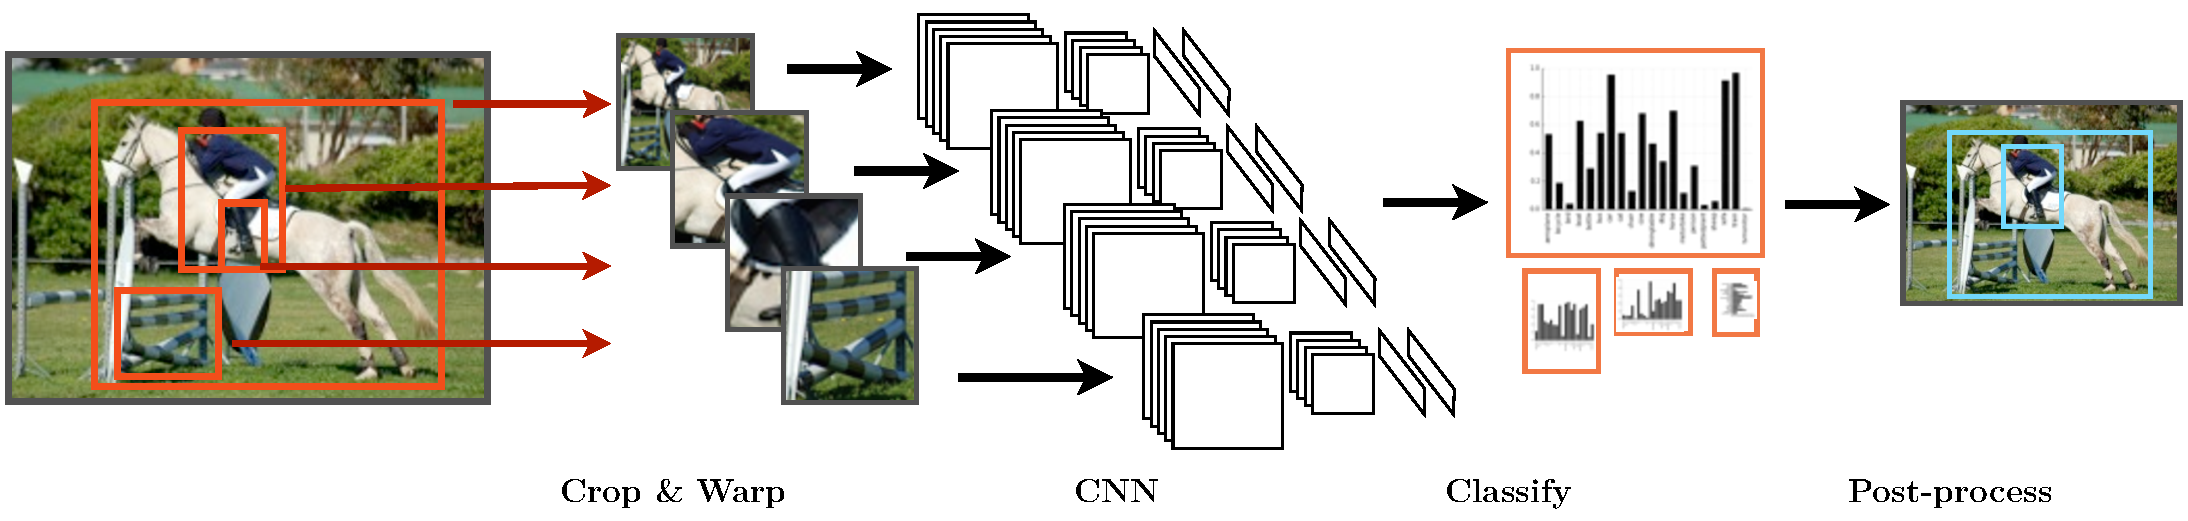
\includegraphics[width=0.98\columnwidth]{../ccnn/figures/rcnn.pdf}
\caption{
R-CNN architecture: image regions are cropped, resized, and each one fed through a CNN.
The classifier outputs are post-processed to give the final detections.
}\label{fig:rcnn}
\end{center}
\end{figure}


\begin{figure}[ht]
\begin{center}
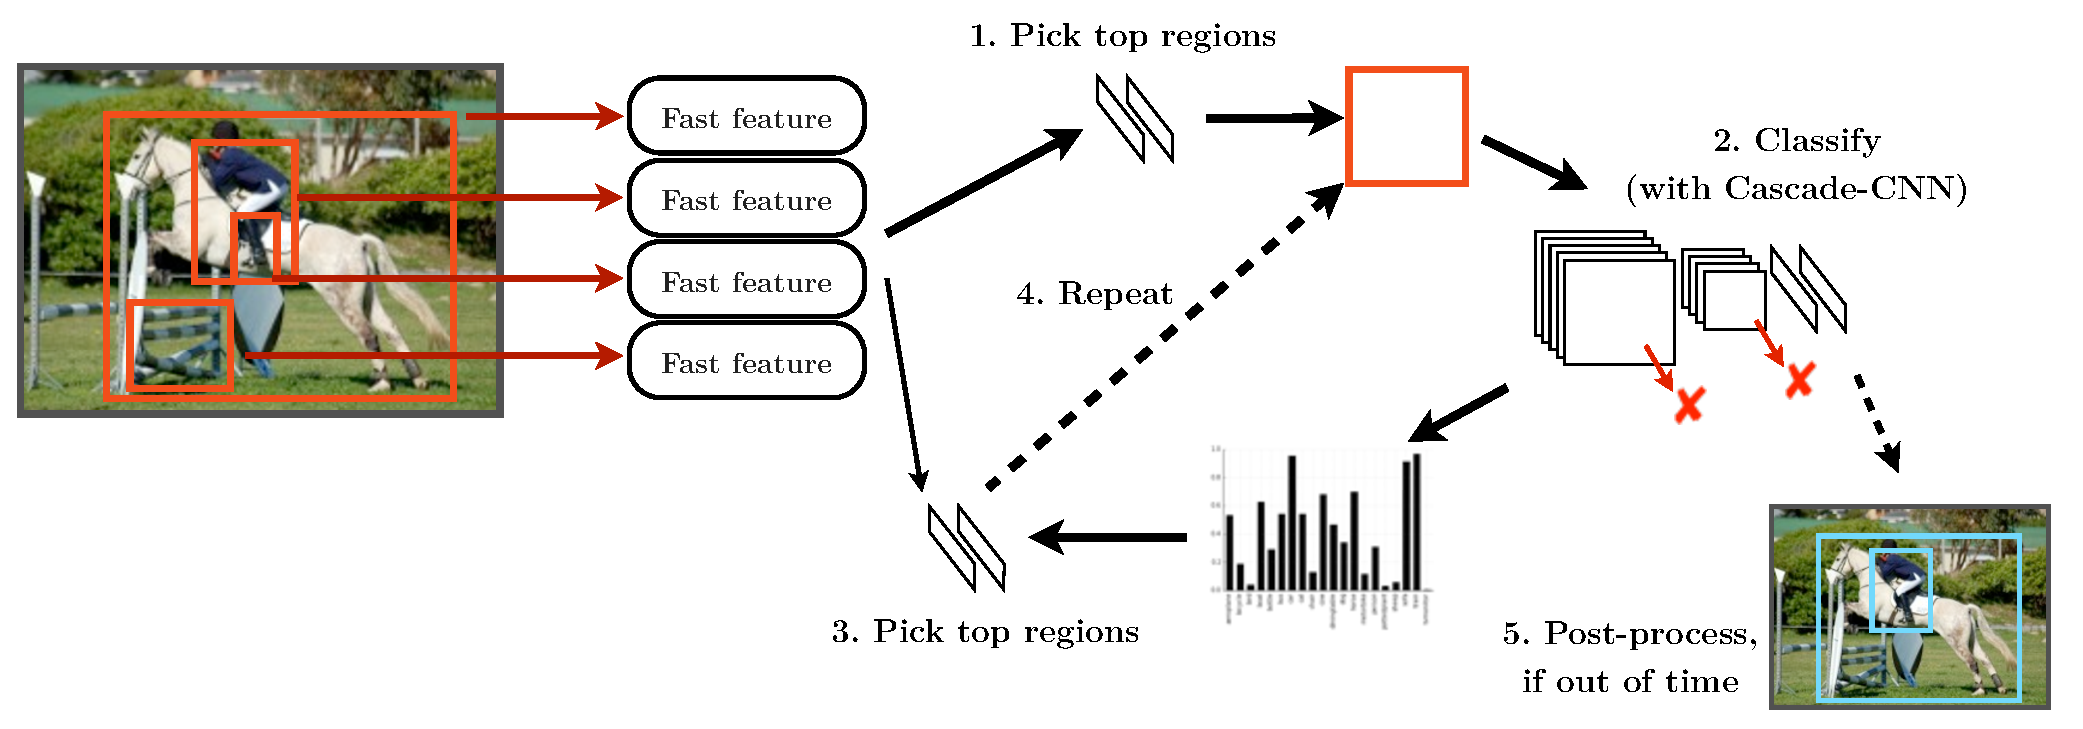
\includegraphics[width=0.98\columnwidth]{../ccnn/figures/combined.pdf}
\caption{
Our method scores each region of interest with a fast feature (we evaluate several), allowing us to pick promising regions first.
The regions are classified with the original CNN, or a sped-up Cascade-CNN.
The properties of the regions can play a role in selecting the next batch of regions.
}\label{fig:combined}
\end{center}
\end{figure}


\subsection{Quick-to-compute feature}

\PM{Region statistics}
For the first source of information, we consider statistics about ROI location and overlap with other regions.
For each ROI, we compute: its normalized location, its scale ($\sqrt{\text{width} \times \text{height}}$), aspect ratio ($\log \sqrt{\text{width} / \text{height}}$), and normalized counts of overlapping regions, at several PASCAL overlap thresholds (0, 0.2, 0.6).
This simple feature works suprisingly well for filtering regions to process first.

\PM{Pixel gradient}
In concatenation, we also consider the \emph{pixel gradient}, back-propagated throgh a classification CNN applied to the whole image.
This feature corresponds to a kind of saliency map, giving an estimate of the importance of each pixel to the final classification of the image.
Our method follows \cite{Simonyan-ICLR-2014} to the best of our knowledge.
Images are resized to square and classified with an ``AlexNet'' \cite{Krizhevsky-NIPS-2012} CNN fine-tuned on the PASCAL VOC classification dataset with multi-label loss.
(Unlike the ILSVRC, the PASCAL VOC is a multi-label prediction task, with at times multiple correct labels for an image.)
At test-time, the gradient at the top is with respect to the indicator function of the max-scoring class, and is back-propagated all the way to the pixels, where it is summed across channels.
A couple of example images are shown in \autoref{fig:gradient_examples}.
We compute an integral image on this pixel gradient map, allowing near-instant computation of sums in arbitrary regions.
For each region to be evaluated, we compute the image-normalized gradient sum, sums for each of four corners, and ratio of in-region vs. out-of-region sums.

\begin{figure}
\centering
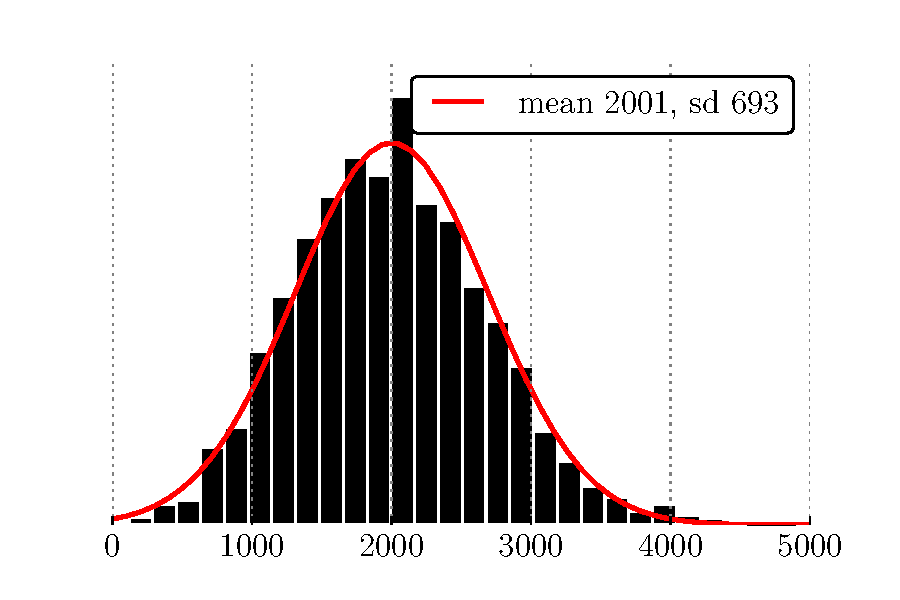
\includegraphics[width=\linewidth]{../ccnn/figures/roi_hist.pdf}
\caption{
Distribution of number of regions per image.
}\label{fig:roi_hist}
\end{figure}

\begin{figure}
\centering
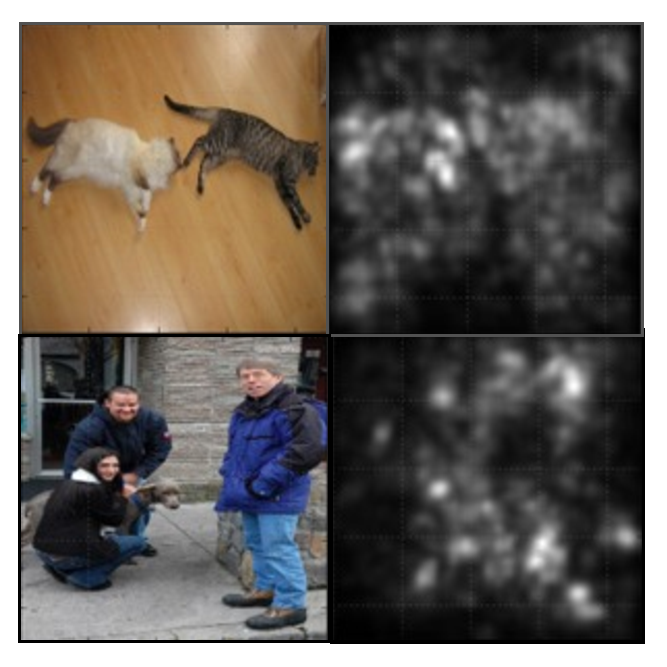
\includegraphics[width=\linewidth]{../ccnn/figures/gradient.pdf}
\caption{
Two different examples of the CNN gradient that we use as a quick-to-compute feature.
}\label{fig:gradient_examples}
\end{figure}

\subsection{Cascaded CNN}\label{sec:ccnn}

\PM{Motivation}
Despite the intentions of the region-proposal mechanism \parencite{Uijlings-IJCV-2013}, most ROIs that are scored in R-CNN do not contain any object of interest.
As in the classic cascade of \cite{Viola-IJCV-2004}, it would be useful to quickly reject these regions, without expending the full amount of computation on them.
The problem is that the deep neural network architecture is trained to always run all the way through.
We need to introduce a new primitive to enable early termination.

\PM{Method}
The Cascaded CNN, shown in \autoref{fig:ccnn}, augments the CNN network with an ``Early Reject'' option: after some layers, the network decides whether to keep processing the input with the next layer.
Each reject layer is implemented as a fully-connected layer following a linear rectification, trained with dropout using logistic loss on foreground/background labels.
We first train an AlexNet-architecture network \parencite{Krizhevsky-NIPS-2012} on the ImageNet classification dataset.
This network is augmented with the Reject layers, its loss replaced with a multi-label cross-entropy loss, and fine-tuning on the PASCAL VOC training set is performed until loss stop decreasing (roughly 50000 iterations).
In training, all instances pass through all Reject layers.
After training, we set the reject thresholds to maintain at last 80\% recall at each stage, using a large sample of regions from images in the validation set containing positive and negative examples in equal proportion.

\PM{Implementation}
In the efficient implementation of CNNs we use (Caffe), there is a simple loop over each batch element in both CPU and GPU convolution code.
We modify this loop to simply not perform convolution on those elements that were rejected earlier in the cascade.
\footnote{While memory remains occupied in this scheme, we do not consider this a problem.}
Since most of the time is spent in the convolutional layers, we introduce a reject option after \texttt{pool1}, \texttt{pool2}, and \texttt{conv3}.
The last classification layer still outputs the full multi-class scores for the surviving regions.

\PM{Timing}
To estimate the saving on time by using the rejectors we timed the time spend to process 1000 regions (10 batches or 100) and the time expended in each of the first 3 layers:
\begin{itemize}
\item 1700 ms to process all the layers
\item 270 ms (15\%) in layer 1 (This includes \texttt{conv1}, \texttt{relu1}, \texttt{pool1}, \texttt{norm1})
\item 360 ms (20\%) in layer 2 (This includes \texttt{conv2}, \texttt{relu2}, \texttt{pool2}, \texttt{norm2})
\item 285 ms (15\%) in layer 3 (This includes \texttt{conv3}, \texttt{relu3})
\end{itemize}
Therefore the expected ``lifetimes'' of regions rejected after layer 1, layer 2, and layer 3 are  0.15, 0.35, and 0.5 of the total time taken per region.

\begin{figure}[h!]
\begin{center}
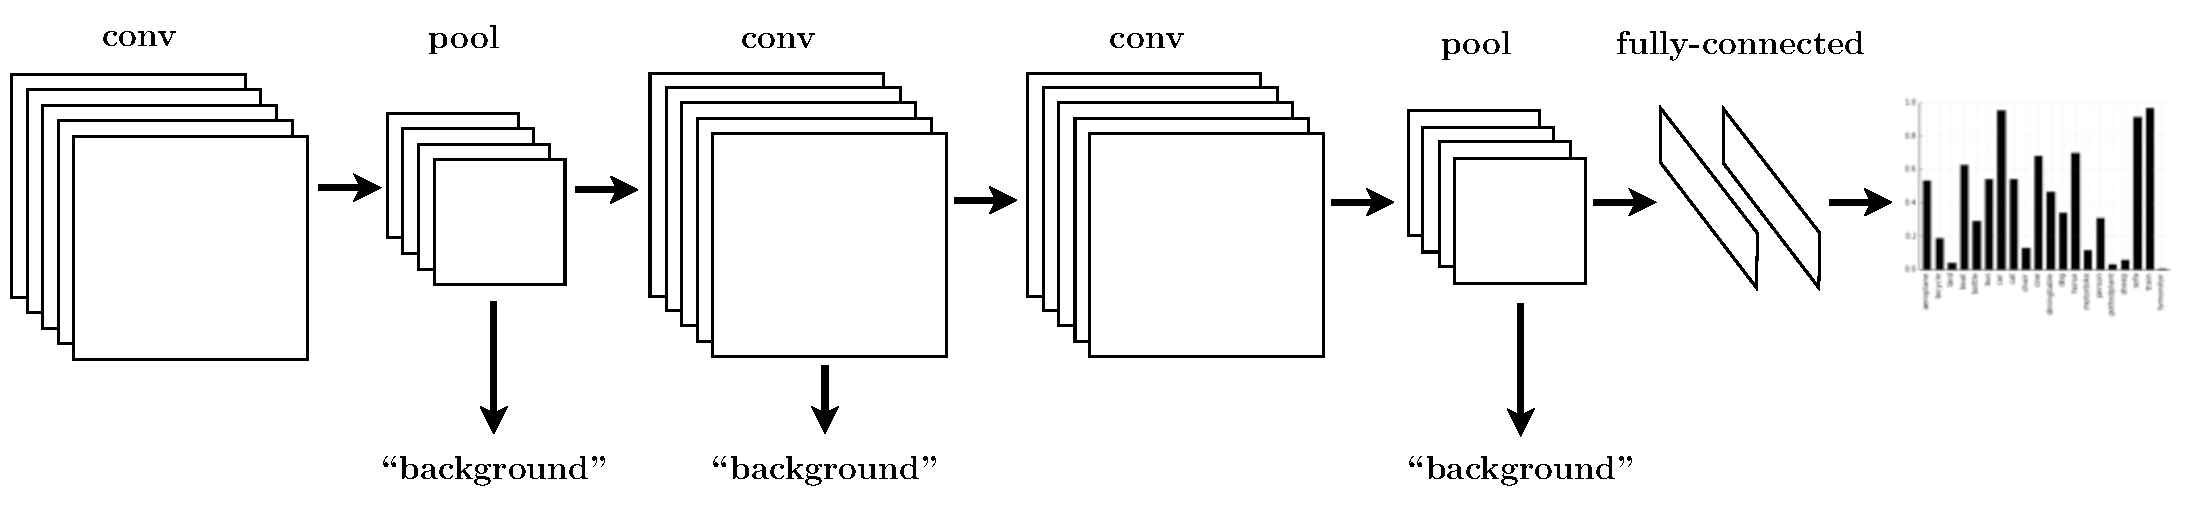
\includegraphics[width=0.98\columnwidth]{../ccnn/figures/ccnn.pdf}
\caption{
The Cascaded CNN has a reject option after pool1, pool2 and conv3 layers.
}\label{fig:ccnn}
\end{center}
\end{figure}

